\documentclass[11pt,a4paper]{article}

\usepackage[margin=2.5cm]{geometry}
\usepackage{amsmath,amssymb}
\usepackage{bm}
\usepackage{enumitem}
\usepackage{hyperref}
\usepackage{tikz}
\usetikzlibrary{arrows.meta,positioning,shapes.geometric}

\title{Sequence Comparison Tools}
\author{CBBL Tools}
\date{\today}

\tikzset{
  methodbox/.style={
    rounded corners=6pt,
    draw=blue!50!black,
    line width=0.9pt,
    fill=blue!6,
    minimum width=13cm,
    text width=11.8cm,
    align=left,
    inner sep=8pt
  }
}

\begin{document}
\maketitle

\tableofcontents

\section{Scope}

This folder contains eight notebooks that start from the same FASTA inputs and represent sequence relationships in different mathematical ways:

\begin{itemize}[leftmargin=*]
\item \texttt{ternary\_alignment\_substitution.ipynb}
\item \texttt{kras\_msa\_publication.ipynb}
\item \texttt{sequence\_similarity\_network.ipynb}
\item \texttt{ternary\_hamming.ipynb}
\item \texttt{ternary\_levenshtein.ipynb}
\item \texttt{trilateration\_hamming.ipynb}
\item \texttt{mds\_levenshtein.ipynb}
\item \texttt{kmer\_pca.ipynb}
\end{itemize}

The first notebook is a reference-based ternary map built from alignment scores, the second is a publication-oriented MSA visualization workflow, the third is a sequence similarity network analysis, the fourth and fifth are simpler reference-based ternary maps, the sixth is a reference-based trilateration embedding, the seventh is a global distance-matrix ordination, and the eighth is a feature-based compositional ordination.

\section{Input model}

All notebooks use the same logical setup:

\begin{itemize}[leftmargin=*]
\item a FASTA file with exactly three reference sequences $A$, $B$, and $C$,
\item a FASTA file with additional query sequences $Q_1,\dots,Q_n$.
\end{itemize}

For any query $Q$, the basic reference-based quantities are
\[
d_A(Q)=d(Q,A),\qquad d_B(Q)=d(Q,B),\qquad d_C(Q)=d(Q,C),
\]
or, in similarity form,
\[
s_A(Q),\qquad s_B(Q),\qquad s_C(Q).
\]

Depending on the notebook, these quantities are turned into:

\begin{itemize}[leftmargin=*]
\item a ternary composition of relative similarity,
\item a trilaterated point in the plane,
\item a full pairwise distance matrix for ordination,
\item or a feature vector built from $k$-mer compositions.
\end{itemize}

\section{Distance and similarity functions}

\subsection{Normalized Hamming distance}

If two sequences $X$ and $Y$ have the same length $L$, the normalized Hamming distance is
\[
d_{\mathrm{Ham}}(X,Y)=\frac{1}{L}\sum_{k=1}^{L}\mathbf{1}\{X_k\neq Y_k\}.
\]

This is the fraction of mismatching positions. It is simple and interpretable, but requires aligned or at least position-wise comparable sequences of equal length, and it gives every mismatch the same cost.

\subsection{Normalized Levenshtein distance}

For sequences of arbitrary lengths, let $\operatorname{Lev}(X,Y)$ denote the edit distance, i.e. the minimum number of insertions, deletions, and substitutions needed to transform $X$ into $Y$. The normalized form used in the notebooks is
\[
d_{\mathrm{Lev}}(X,Y)=\frac{\operatorname{Lev}(X,Y)}{\max(|X|,|Y|)}.
\]

This allows indels and makes distances comparable across different lengths, but substitutions still all have unit cost.

\subsection{Normalized alignment distance with a substitution matrix}

For homologous sequences, especially proteins, a more informative comparison is obtained from an optimal pairwise alignment score $S(X,Y)$ computed with

\begin{itemize}[leftmargin=*]
\item a global alignment algorithm such as Needleman--Wunsch when full-length homology is expected,
\item or a local alignment algorithm such as Smith--Waterman when only a conserved region should drive the comparison,
\item a substitution matrix,
\item affine gap penalties.
\end{itemize}

For proteins, the standard practical default is BLOSUM62 with affine gaps. A strong normalized dissimilarity is
\[
d_{\mathrm{align}}(X,Y)=1-\frac{S(X,Y)}{\sqrt{S(X,X)\,S(Y,Y)}}.
\]

Equivalently,
\[
s_{\mathrm{align}}(X,Y)=\frac{S(X,Y)}{\sqrt{S(X,X)\,S(Y,Y)}}
\]
is a normalized alignment similarity. This normalization ensures $d_{\mathrm{align}}(X,X)=0$ and partially adjusts for sequence length and composition through self-scores.

An alternative baseline normalization is
\[
d(X,Y)=1-\frac{S(X,Y)-S_{\min}}{S_{\max}-S_{\min}},
\]
but the self-score normalization above is often the simplest useful default in practice.

\subsection{Why alignment-based similarity is often better for proteins}

Hamming and Levenshtein treat all substitutions equally. Biologically, however, an Ile$\leftrightarrow$Leu replacement is usually milder than a Trp$\leftrightarrow$Gly replacement. A substitution matrix incorporates these differential costs. Therefore alignment-based similarity is typically preferable for proteins whenever the sequences are alignable.

\subsection{Sequence-type recommendations}

\begin{itemize}[leftmargin=*]
\item For proteins: global alignment with BLOSUM62 and affine gaps is the default recommendation for the ternary workflow.
\item For DNA/RNA: a substitution matrix can be used operationally, but model-based nucleotide distances such as Jukes--Cantor or Kimura are often more principled when the goal is evolutionary interpretation.
\item For highly diverged, rearranged, recombinant, or very large sequence collections: feature-based or alignment-free methods may be more robust.
\end{itemize}

\subsection{Important caveat}

A raw alignment score is not automatically a metric. Triangle inequality may fail, normalization choices matter, and gap penalties affect geometry. For the visual tools in this folder, what is required is a consistent dissimilarity, not necessarily a strict metric in the formal sense.

\section{Notebook 1: ternary mapping from normalized alignment distance}

\subsection{Distance-to-similarity model}

The notebook \texttt{ternary\_alignment\_substitution.ipynb} computes pairwise alignment scores with \texttt{Biopython}'s \texttt{PairwiseAligner}, affine gap penalties, and the substitution matrix BLOSUM62. The notebook is now intentionally specialized to homologous protein sequences and uses a bundled K-RAS protein example by default.

For any query $Q$, define
\[
s_A(Q)=s_{\mathrm{align}}(Q,A),\qquad
s_B(Q)=s_{\mathrm{align}}(Q,B),\qquad
s_C(Q)=s_{\mathrm{align}}(Q,C),
\]
where
\[
s_{\mathrm{align}}(X,Y)=\frac{S(X,Y)}{\sqrt{S(X,X)\,S(Y,Y)}}.
\]

The corresponding distance is
\[
d_i(Q)=1-s_i(Q),\qquad i\in\{A,B,C\}.
\]

\subsection{Closure into a ternary composition}

The three normalized similarities are closed into
\[
\lambda_i(Q)=\frac{s_i(Q)}{s_A(Q)+s_B(Q)+s_C(Q)},\qquad i\in\{A,B,C\}.
\]

Hence
\[
\bm{\lambda}(Q)=\big(\lambda_A(Q),\lambda_B(Q),\lambda_C(Q)\big)
\]
is a 3-part composition satisfying
\[
\lambda_A(Q)+\lambda_B(Q)+\lambda_C(Q)=1,\qquad \lambda_i(Q)\ge 0.
\]

\subsection{Barycentric map into the triangle}

The triangle vertices are fixed as
\[
V_A=(0,0),\qquad
V_B=(1,0),\qquad
V_C=\left(\frac12,\frac{\sqrt3}{2}\right).
\]

The plotted point is
\[
\bm{p}(Q)=\lambda_A(Q)V_A+\lambda_B(Q)V_B+\lambda_C(Q)V_C.
\]

\subsection{Interpretation}

This is the biologically strongest ternary notebook in the folder for homologous protein sequences. Still, the plotted point should be read as a \emph{relative allocation of normalized alignment similarity} to the three references, not as an exact Euclidean preservation of the three underlying dissimilarities.

\section{Notebook 2: publication-quality MSA visualization of K-RAS homologs}

\subsection{Input design}

The notebook \texttt{kras\_msa\_publication.ipynb} uses the FASTA file \texttt{kras\_homologs\_10.fasta}, which contains ten homologous K-RAS proteins from UniProt. The first sequence is the human K-RAS protein and acts as the reference for alignment coordinates and residue numbering.

\subsection{Reference-guided alignment construction}

Let the reference sequence be $R=r_1,\dots,r_L$ and let $X_1,\dots,X_n$ be the homologous proteins. For each sequence $X_i$, the notebook computes a global pairwise alignment against $R$ using BLOSUM62 and affine gap penalties. This yields:

\begin{itemize}[leftmargin=*]
\item aligned residue assignments to each reference position,
\item insertion strings between consecutive reference residues.
\end{itemize}

For each boundary $j\in\{0,\dots,L\}$, let $I_i(j)$ denote the insertion segment of sequence $X_i$ between reference positions $j$ and $j+1$ (with $j=0$ before the first reference residue and $j=L$ after the last one). The notebook defines the insertion capacity
\[
m_j=\max_{i=1,\dots,n}|I_i(j)|.
\]

The final multiple alignment is assembled by padding each insertion slot to length $m_j$. Thus each aligned sequence is written in a common coordinate system consisting of:

\begin{itemize}[leftmargin=*]
\item an insertion block of width $m_0$,
\item reference position $1$,
\item an insertion block of width $m_1$,
\item reference position $2$,
\item and so on until reference position $L$ and the tail insertion block of width $m_L$.
\end{itemize}

This is a reference-guided progressive construction rather than a full de novo MSA optimization.

\subsection{Consensus and conservation}

If the aligned column $k$ contains residue counts $n_k(a)$ over the non-gap alphabet, the notebook defines the consensus residue as the most frequent non-gap symbol and the conservation score as
\[
c_k=\frac{\max_a n_k(a)}{\sum_a n_k(a)}.
\]

Hence $c_k\in[0,1]$, with $c_k=1$ for a fully conserved non-gap column.

\subsection{Visualization}

The figure combines:

\begin{itemize}[leftmargin=*]
\item residue-class coloring,
\item monospace residue labels,
\item a per-column conservation bar,
\item a consensus row,
\item and annotated K-RAS regions such as the P-loop, Switch~I, Switch~II, and the hypervariable C-terminal tail.
\end{itemize}

This notebook is intended for close inspection of a small homologous protein family, not for low-dimensional embedding.

\section{Notebook 3: sequence similarity network from a FASTA file}

\subsection{Weighted similarity graph}

The notebook \texttt{sequence\_similarity\_network.ipynb} starts from a FASTA file of homologous proteins and computes all pairwise normalized alignment similarities
\[
w_{ij}=\frac{A(S_i,S_j)}{\sqrt{A(S_i,S_i)\,A(S_j,S_j)}},
\]
where $A(S_i,S_j)$ is the global alignment score obtained from \texttt{Biopython PairwiseAligner} with BLOSUM62 and affine gaps.

This yields a symmetric similarity matrix
\[
W=(w_{ij})_{i,j=1}^n,\qquad w_{ii}=1.
\]

\subsection{Thresholded sequence similarity network}

For a chosen threshold $\tau\in[0,1]$, the SSN is the weighted graph
\[
G_\tau=(V,E_\tau),\qquad V=\{1,\dots,n\},
\]
with
\[
(i,j)\in E_\tau \iff w_{ij}\ge \tau.
\]

When an edge is present, its weight is the retained similarity itself:
\[
\omega(i,j)=w_{ij}.
\]

Thus the network is a filtered version of the full similarity matrix. Increasing $\tau$ produces a sparser graph and reveals finer neighborhoods; decreasing $\tau$ merges neighborhoods into larger connected components.

\subsection{Interpretation}

This notebook is well suited to the exploration of local neighborhoods in sequence space, which is one of the main practical uses of SSNs in protein family analysis. Connected components, hubs, and dense subnetworks may indicate candidate subfamilies or groups of functionally related sequences.

However, the 2D graph layout used for plotting is only a visualization device. It is not a metric embedding and it is not a phylogenetic tree.

\section{Notebook 4: ternary mapping from Hamming distance}

\subsection{Distance-to-similarity map}

The notebook \texttt{ternary\_hamming.ipynb} starts from
\[
d_A(Q),\quad d_B(Q),\quad d_C(Q)
\]
computed with normalized Hamming distance and transforms them into nonnegative similarity scores
\[
s_A(Q)=\max(0,1-d_A(Q)),\qquad
s_B(Q)=\max(0,1-d_B(Q)),\qquad
s_C(Q)=\max(0,1-d_C(Q)).
\]

\subsection{Closure and barycentric mapping}

The three scores are closed into
\[
\lambda_i(Q)=\frac{s_i(Q)}{s_A(Q)+s_B(Q)+s_C(Q)},\qquad i\in\{A,B,C\},
\]
and then mapped with the same barycentric triangle formula
\[
\bm{p}(Q)=\lambda_A(Q)V_A+\lambda_B(Q)V_B+\lambda_C(Q)V_C.
\]

\subsection{Interpretation}

This notebook is a simple baseline. It is appropriate only when equal-length, position-wise comparison already captures the intended biological relation.

\section{Notebook 5: ternary mapping from Levenshtein distance}

The notebook \texttt{ternary\_levenshtein.ipynb} has the same mathematical structure as the Hamming-based one, but replaces
\[
d_i(Q)=d_{\mathrm{Ham}}(Q,i)
\]
with
\[
d_i(Q)=d_{\mathrm{Lev}}(Q,i),\qquad i\in\{A,B,C\}.
\]

Then it applies the same distance-to-similarity transform, the same closure, and the same barycentric map.

Its advantage over Hamming is robustness to unequal lengths and indels. Its disadvantage relative to alignment scoring is that all substitutions still have equal cost.

\section{Why the ternary representation is limited}

This part is central, because all three ternary notebooks are useful but mathematically limited.

\subsection{1. They do not preserve the real sequence distances}

The map
\[
(d_A,d_B,d_C)\mapsto (s_A,s_B,s_C)\mapsto
\left(
\frac{s_A}{s_A+s_B+s_C},
\frac{s_B}{s_A+s_B+s_C},
\frac{s_C}{s_A+s_B+s_C}
\right)
\]
is many-to-one. Information is lost.

Therefore the triangle is not a metric embedding of sequence space.

\subsection{2. The triangle encodes only relative proportions}

Because
\[
\lambda_A+\lambda_B+\lambda_C=1,
\]
the representation only preserves relative allocation among the three references.

Two sequences may have very different absolute distance scales and still end up at the same ternary position if their transformed similarity ratios are the same.

\subsection{3. The result depends critically on the transform $d\mapsto s$}

The geometry depends on how dissimilarities are converted to nonnegative similarities. Even if the Hamming and Levenshtein notebooks use
\[
s=\max(0,1-d),
\]
and the alignment notebook uses a normalized score
\[
s=\frac{S(X,Y)}{\sqrt{S(X,X)\,S(Y,Y)}},
\]
other transformations would generate different maps. Hence the representation is not invariant.

\subsection{4. The map depends strongly on the chosen references}

The three references define the coordinate system. Changing $A$, $B$, or $C$ changes the whole ternary geometry. This is a landmark-type construction, not an intrinsic embedding of the full dataset.

\subsection{5. The triangle is not a phylogenetic geometry}

A point close to side $AB$ does \emph{not} imply that the sequence is evolutionarily between $A$ and $B$. That visual pattern may arise from many causes: shared ancestry, convergence, saturation, or simply the chosen distance definition.

\subsection{6. This is not strict CoDA on original data}

In classical compositional data analysis, the parts are components of a common whole. Here the raw inputs are distances or similarities to three references, not literal parts of one total. The compositional structure is introduced by modeling choice after converting these quantities into nonnegative affinities and applying closure.

So the simplex viewpoint is appropriate for \emph{relative similarity}, not because the original sequence measurements are themselves compositions.

\section{Notebook 6: distance-based trilateration}

\subsection{Geometric idea}

The notebook \texttt{trilateration\_hamming.ipynb} takes the three reference points
\[
V_A,\quad V_B,\quad V_C\in\mathbb{R}^2
\]
and looks for a point $\bm{z}(Q)$ such that
\[
\|\bm{z}(Q)-V_A\|_2\approx d_A(Q),\qquad
\|\bm{z}(Q)-V_B\|_2\approx d_B(Q),\qquad
\|\bm{z}(Q)-V_C\|_2\approx d_C(Q).
\]

This is the same mathematical structure as trilateration in localization problems.

\subsection{Linearized equations}

Starting from
\[
\|\bm{z}-V_A\|_2^2=d_A^2,\qquad
\|\bm{z}-V_B\|_2^2=d_B^2,\qquad
\|\bm{z}-V_C\|_2^2=d_C^2,
\]
subtracting the first equation from the second and third yields
\[
2(V_B-V_A)^\top \bm{z}
=d_A^2-d_B^2+\|V_B\|_2^2-\|V_A\|_2^2,
\]
\[
2(V_C-V_A)^\top \bm{z}
=d_A^2-d_C^2+\|V_C\|_2^2-\|V_A\|_2^2.
\]

This can be written as
\[
M\bm{z}=\bm{r},
\]
with
\[
M=
2\begin{bmatrix}
(V_B-V_A)^\top \\
(V_C-V_A)^\top
\end{bmatrix}.
\]

The notebook solves this system by least squares.

\subsection{Residuals}

Since sequence distances are rarely perfectly realizable in a 2D Euclidean anchor system, the notebook also reports residuals
\[
\rho_i(Q)=\left|\|\bm{z}(Q)-V_i\|_2-d_i(Q)\right|,
\qquad i\in\{A,B,C\},
\]
and their mean.

\subsection{Interpretation}

This approach is more faithful to actual distance magnitudes than ternary closure, but it still inherits the quality and limitations of the chosen distance function. In particular, if the distance model is too crude, the trilateration cannot repair that upstream weakness.

\section{Notebook 7: classical MDS from the full distance matrix}

\subsection{Distance matrix}

The notebook \texttt{mds\_levenshtein.ipynb} uses all references and all queries together. If
\[
\{S_1,\dots,S_N\}=\{A,B,C,Q_1,\dots,Q_n\},
\]
then the pairwise distance matrix is
\[
\Delta=(\delta_{ij})_{i,j=1}^{N},
\qquad
\delta_{ij}=d_{\mathrm{Lev}}(S_i,S_j).
\]

\subsection{Double-centering step}

Classical MDS builds a Gram-type matrix from squared distances:
\[
J=I_N-\frac{1}{N}\bm{1}\bm{1}^\top,
\]
\[
B=-\frac12 J\Delta^{\circ 2}J,
\]
where $\Delta^{\circ 2}$ denotes elementwise squaring.

\subsection{Spectral embedding}

If
\[
B=U\Lambda U^\top
\]
is the eigendecomposition, then the 2D coordinates are
\[
X_2=U_2\Lambda_2^{1/2},
\]
where $U_2$ contains the first two eigenvectors associated with the largest nonnegative eigenvalues.

\subsection{Interpretation}

Unlike the ternary or trilateration notebooks, MDS is a global distance-based ordination. It does not privilege the three references except that they are included as part of the dataset.

Its target is not relative similarity to three anchors but approximate preservation of the full pairwise distance geometry. The same MDS construction could also be paired with a matrix of normalized alignment distances if protein-aware geometry is needed globally.

\section{Notebook 8: PCA on clr-transformed $k$-mer compositions}

\subsection{From sequences to compositions}

The notebook \texttt{kmer\_pca.ipynb} does not start from edit distances. Instead, each sequence is converted into a composition of $k$-mer frequencies.

Let $\mathcal{A}$ be the alphabet and let
\[
D=|\mathcal{A}|^k
\]
be the number of possible $k$-mers. If $n_j(S)$ is the count of the $j$-th $k$-mer in sequence $S$, and $\alpha>0$ is a pseudocount, define
\[
\tilde{n}_j(S)=n_j(S)+\alpha.
\]

The closed composition is
\[
x_j(S)=\frac{\tilde{n}_j(S)}{\sum_{m=1}^{D}\tilde{n}_m(S)}.
\]

Thus
\[
\bm{x}(S)=\big(x_1(S),\dots,x_D(S)\big)
\]
lives in the simplex.

\subsection{Centered log-ratio transform}

To move from the simplex to a Euclidean coordinate system, the notebook applies the centered log-ratio transform
\[
\operatorname{clr}(\bm{x})=
\left(
\log\frac{x_1}{g(\bm{x})},
\dots,
\log\frac{x_D}{g(\bm{x})}
\right),
\]
where
\[
g(\bm{x})=\left(\prod_{j=1}^{D}x_j\right)^{1/D}
\]
is the geometric mean.

\subsection{PCA}

Let
\[
Z\in\mathbb{R}^{N\times D}
\]
be the matrix whose rows are the clr vectors for all sequences. After column centering,
\[
Z_c=Z-\bm{1}\bar{\bm{z}}^\top,
\]
PCA is obtained from the singular value decomposition
\[
Z_c=U\Sigma V^\top.
\]

The first two principal component scores are
\[
T_2=Z_cV_2.
\]

\subsection{Interpretation}

This notebook is not a distance embedding. It is a feature-based ordination that captures dominant variation in compositional sequence content. It is often preferable when alignments are unstable or when local compositional signal matters more than explicit sitewise homology.

\section{Optional note on Aitchison geometry}

The ternary coordinates
\[
\bm{\lambda}(Q)=\big(\lambda_A(Q),\lambda_B(Q),\lambda_C(Q)\big)
\]
live in the simplex
\[
\mathcal{S}^3=\left\{\bm{x}\in\mathbb{R}_+^3:\sum_{i=1}^{3}x_i=1\right\}.
\]

If ternary points are compared quantitatively, the natural geometry is Aitchison geometry, not ordinary Euclidean geometry on raw parts. The Aitchison distance is
\[
d_{\mathrm{Ait}}(\bm{x},\bm{y})
=\left\|\operatorname{clr}(\bm{x})-\operatorname{clr}(\bm{y})\right\|_2.
\]

This matters because Euclidean distances between plotted points in the triangle are not the same thing as compositional distances in the simplex.

\section{When each notebook is appropriate}

\begin{itemize}[leftmargin=*]
\item Use \texttt{ternary\_alignment\_substitution.ipynb} as the default reference-based notebook for homologous protein sequences.
\item Use \texttt{kras\_msa\_publication.ipynb} when the goal is to inspect residue-level conservation, local divergence, and functional regions in a small homologous protein family.
\item Use \texttt{sequence\_similarity\_network.ipynb} when the main question is neighborhood structure, thresholded similarity connectivity, or subfamily detection in sequence space.
\item Use \texttt{ternary\_hamming.ipynb} only when all sequences have equal length and position-wise mismatches are already the intended comparison model.
\item Use \texttt{ternary\_levenshtein.ipynb} when indels and unequal lengths matter but you still want a simple reference-relative edit-distance baseline.
\item Use \texttt{trilateration\_hamming.ipynb} when you want a more literal anchor-based distance reconstruction in 2D.
\item Use \texttt{mds\_levenshtein.ipynb} when the global pairwise geometry of the whole dataset matters most.
\item Use \texttt{kmer\_pca.ipynb} when sequence composition and motif-like content are more relevant than direct alignment or edit distances.
\end{itemize}

\section{Method scheme}

Figure~\ref{fig:summary} summarizes the conceptual relations between the eight notebooks.

\begin{figure}[ht]
\centering
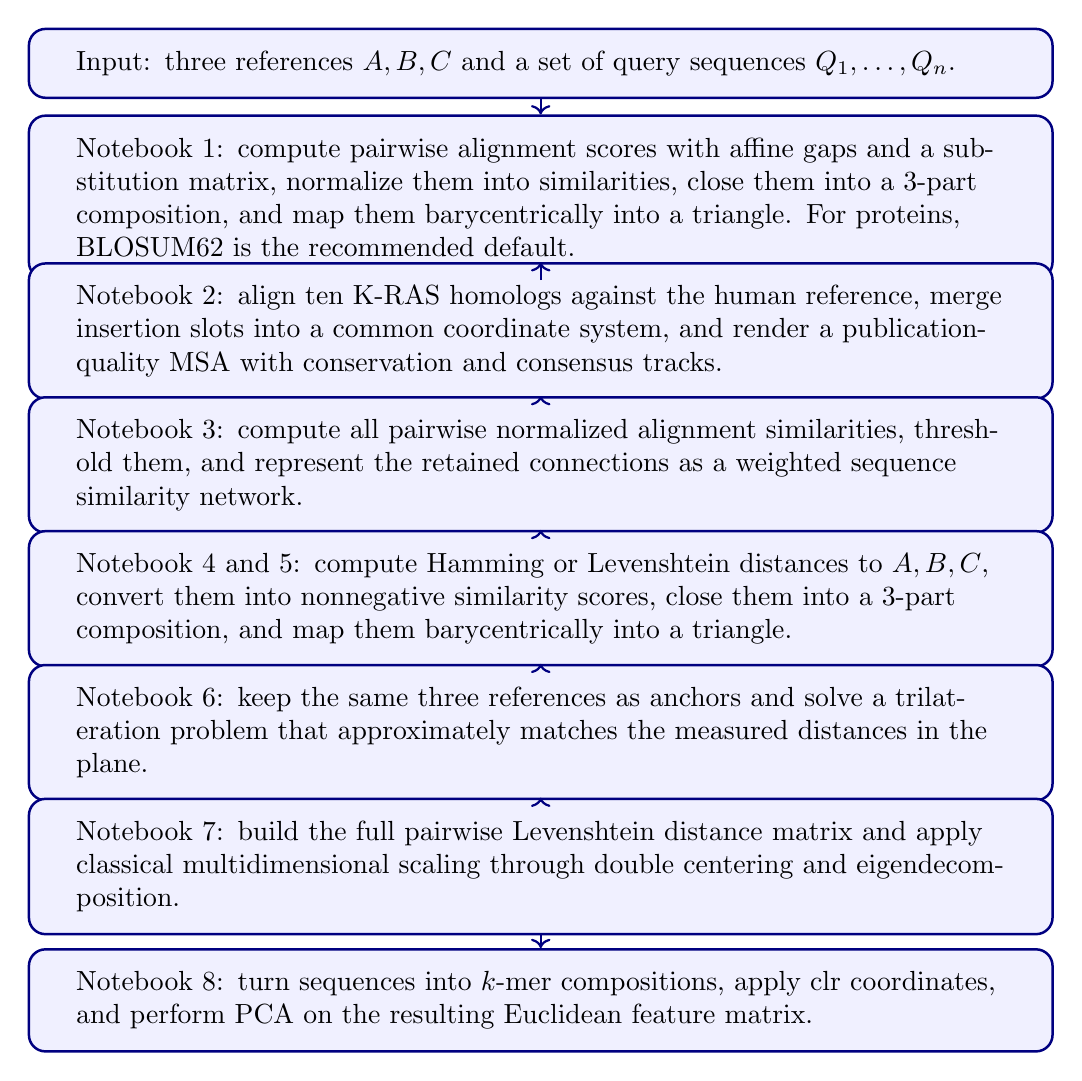
\begin{tikzpicture}[x=1cm,y=1cm]
\node[methodbox] (m0) at (0,0.0) {Input: three references $A,B,C$ and a set of query sequences $Q_1,\dots,Q_n$.};
\node[methodbox] (m1) at (0,-1.7) {Notebook 1: compute pairwise alignment scores with affine gaps and a substitution matrix, normalize them into similarities, close them into a 3-part composition, and map them barycentrically into a triangle. For proteins, BLOSUM62 is the recommended default.};
\node[methodbox] (m2) at (0,-3.4) {Notebook 2: align ten K-RAS homologs against the human reference, merge insertion slots into a common coordinate system, and render a publication-quality MSA with conservation and consensus tracks.};
\node[methodbox] (m3) at (0,-5.1) {Notebook 3: compute all pairwise normalized alignment similarities, threshold them, and represent the retained connections as a weighted sequence similarity network.};
\node[methodbox] (m4) at (0,-6.8) {Notebook 4 and 5: compute Hamming or Levenshtein distances to $A,B,C$, convert them into nonnegative similarity scores, close them into a 3-part composition, and map them barycentrically into a triangle.};
\node[methodbox] (m5) at (0,-8.5) {Notebook 6: keep the same three references as anchors and solve a trilateration problem that approximately matches the measured distances in the plane.};
\node[methodbox] (m6) at (0,-10.2) {Notebook 7: build the full pairwise Levenshtein distance matrix and apply classical multidimensional scaling through double centering and eigendecomposition.};
\node[methodbox] (m7) at (0,-11.9) {Notebook 8: turn sequences into $k$-mer compositions, apply clr coordinates, and perform PCA on the resulting Euclidean feature matrix.};
\draw[->, thick, color=blue!50!black] (m0.south) -- (m1.north);
\draw[->, thick, color=blue!50!black] (m1.south) -- (m2.north);
\draw[->, thick, color=blue!50!black] (m2.south) -- (m3.north);
\draw[->, thick, color=blue!50!black] (m3.south) -- (m4.north);
\draw[->, thick, color=blue!50!black] (m4.south) -- (m5.north);
\draw[->, thick, color=blue!50!black] (m5.south) -- (m6.north);
\draw[->, thick, color=blue!50!black] (m6.south) -- (m7.north);
\end{tikzpicture}
\caption{Conceptual map of the eight sequence-comparison notebooks.}
\label{fig:summary}
\end{figure}

\section{Selected references}

\begin{itemize}[leftmargin=*]
\item J. Aitchison (1986), \emph{The Statistical Analysis of Compositional Data}.
\item V. Pawlowsky-Glahn and A. Buccianti (2011), \emph{Compositional Data Analysis}.
\item S. B. Needleman and C. D. Wunsch (1970), \emph{A General Method Applicable to the Search for Similarities in the Amino Acid Sequence of Two Proteins}.
\item T. F. Smith and M. S. Waterman (1981), \emph{Identification of Common Molecular Subsequences}.
\item S. Henikoff and J. G. Henikoff (1992), \emph{Amino Acid Substitution Matrices from Protein Blocks}.
\item H. J. Atkinson et al. (2009), \emph{Using Sequence Similarity Networks for Visualization of Relationships Across Diverse Protein Superfamilies}.
\item C. J. Gerlt et al. (2015), \emph{Enzyme Function Initiative-Enzyme Similarity Tool (EFI-EST): A Web Tool for Generating Protein Sequence Similarity Networks}.
\item N. Oberg et al. (2023), \emph{EFI-EST, EFI-GNT, and EFI-CGFP: Enzyme Function Initiative Web Resource for Genomic Enzymology Tools}.
\item M. O. Dayhoff, R. M. Schwartz, and B. C. Orcutt (1978), \emph{A Model of Evolutionary Change in Proteins}.
\item S. Karlin and S. F. Altschul (1990), \emph{Methods for Assessing the Statistical Significance of Molecular Sequence Features by Using General Scoring Schemes}.
\item S. F. Altschul et al. (1997), \emph{Gapped BLAST and PSI-BLAST: a New Generation of Protein Database Search Programs}.
\item D.-F. Feng and R. F. Doolittle (1987), \emph{Progressive Sequence Alignment as a Prerequisite to Correct Phylogenetic Trees}.
\item S. E. Brenner, C. Chothia, and T. J. P. Hubbard (1998), \emph{Assessing Sequence Comparison Methods with Reliable Structurally Identified Distant Evolutionary Relationships}.
\item R. C. Edgar (2004), \emph{MUSCLE: Multiple Sequence Alignment with High Accuracy and High Throughput}.
\item V. de Silva and J. B. Tenenbaum (2004), \emph{Sparse Multidimensional Scaling using Landmark Points}.
\item P. Legendre and L. Legendre (2012), \emph{Numerical Ecology}.
\item D. W. Mount (2004), \emph{Bioinformatics: Sequence and Genome Analysis}.
\end{itemize}

\end{document}
